%% Packages initialisation
\documentclass[10pt,compress]{beamer}
\usepackage[utf8]{inputenc}               % Enable UTF-8 compatible typing
\usepackage{hyperref}                     % Interactive PDF
\usepackage{tikz}
\usetikzlibrary{fit,calc,trees,positioning,arrows,chains,shapes.geometric,%
    decorations.pathreplacing,decorations.pathmorphing,shapes,%
    matrix,shapes.symbols,intersections}
\usepackage{gantt}


%% Use the default theme
\usetheme{Madrid}

%% Colours block environment headings
% \useinnertheme{rectangles}
% \mode<beamer>{\setbeamertemplate{blocks}[rounded][shadow=false]} 
% \setbeamercolor{block title}{bg=blue!10,fg=black}
% \makeatletter
% \pgfdeclareverticalshading[lower.bg,upper.bg]{bmb@transition}{200cm}{%
%   color(0pt)=(upper.bg); color(2pt)=(upper.bg); color(4pt)=(upper.bg)}
% \makeatother

%% Enable slide numbering
\makeatletter
\setbeamertemplate{footline}
{
  \leavevmode%
  \hbox{%
  \begin{beamercolorbox}[wd=.3\paperwidth,ht=2.25ex,dp=1ex,left]{author in head/foot}%
    \hspace*{2ex}\usebeamerfont{author in head/foot}\insertshortauthor~~\beamer@ifempty{\insertshortinstitute}{}{(\insertshortinstitute)}
  \end{beamercolorbox}%
  \begin{beamercolorbox}[wd=.5\paperwidth,ht=2.25ex,dp=1ex,center]{title in head/foot}%
    \usebeamerfont{title in head/foot}\insertshorttitle
  \end{beamercolorbox}%
  \begin{beamercolorbox}[wd=.2\paperwidth,ht=2.25ex,dp=1ex,right]{date in head/foot}%
    \usebeamerfont{date in head/foot} \usebeamerfont{date in head/foot}\insertshortdate{}\hfill \insertframenumber /\inserttotalframenumber\hspace*{2ex}
  \end{beamercolorbox}}%
  \vskip0pt%
}
\makeatother

%% Hide navigation buttons
\beamertemplatenavigationsymbolsempty

%% Listings
\usepackage{xcolor}
\usepackage{listings}

\lstset{
 backgroundcolor=\color{white},   % choose the background color; you must add \usepackage{color} or \usepackage{xcolor}
 basicstyle=\ttfamily\small,        % the size of the fonts that are used for the code
 commentstyle=\itshape,
 breakatwhitespace=false,         % sets if automatic breaks should only happen at whitespace
 breaklines=true,                 % sets automatic line breaking
 captionpos=b,                    % sets the caption-position to bottom
 deletekeywords={...},            % if you want to delete keywords from the given language
 escapeinside={§*}{*§},          % if you want to add LaTeX within your code
 extendedchars=true,              % lets you use non-ASCII characters; for 8-bits encodings only, does not work with UTF-8
 frame=none,	                   % adds a frame around the code
 keepspaces=true,                 % keeps spaces in text, useful for keeping indentation of code (possibly needs columns=flexible)
 numbers=none,                    % where to put the line-numbers; possible values are (none, left, right)
 rulecolor=\color{black},         % if not set, the frame-color may be changed on line-breaks within not-black text (e.g. comments (green here))
 showspaces=false,                % show spaces everywhere adding particular underscores; it overrides 'showstringspaces'
 showstringspaces=false,          % underline spaces within strings only
 showtabs=false,                  % show tabs within strings adding particular underscores
 tabsize=2,	                   % sets default tabsize to 2 spaces
 title=\lstname,                   % show the filename of files included with \lstinputlisting; also try caption instead of title
  belowcaptionskip=-1\baselineskip,
  xleftmargin=\parindent
}

\definecolor{darkgreen}{rgb}{0.000000,0.392157,0.000000}
\definecolor{violetred}{rgb}{0.915686,0.125490,0.364706}

% Define Links as a lst-language
\lstdefinelanguage{Links}{% 
  morekeywords={spawn, receive, typename, fun, op, var, if, this, true, false, else, case, switch, handle, handler, shallowhandler, do, sig, spawnAngel, spawnDemon, spawn},%
  sensitive=t, % 
  keywordstyle=\color{red},
  emph={Comp,Player,Bool,Int,GTree,Cheat,Zero,Choose,Rand,Move,Winner,Take,Return,Get,Put,GameState,Alice,Bob,Fail,Nothing,Just,Maybe,Toss,Heads,Tails,Process,Buyer,Coffee,Pay,Cost,Candidate,Stop,PassingComet,CelebritySighting,Float,String,Pid,EProcess,Row,Spawn,Yield,Recv,Send,FreshName,Queue,Dictionary,Myself,Type},
  emphstyle={\color{blue}},
  comment=[l]{\#},% 
  commentstyle={\itshape\color{darkgreen}},%
  escapeinside={(*}{*)},%
  morestring=[d]{"},%
  stringstyle={\color{violetred}}%
 }

% Haskell style
\lstdefinestyle{haskell}{
  language=Haskell,
  basicstyle=\linespread{1.0}\ttfamily\footnotesize,
  literate= {+}{{$+$}}1 {*}{{$*$}}1
            {<=}{{$\leq$}}1 {/=}{{$\neq$}}1 
            {==}{{$\equiv$}}1 {=>}{{$\Rightarrow$}}1
            {->}{{$\to$}}1 {<-}{{$\leftarrow$}}1
            {.}{{$\circ$}}1 {$$}{{\$}}1
}
% Ocaml style
\lstdefinestyle{ocaml}{
  language=Caml,%
  morekeywords={effect, perform},%
  emph={Obj,Choose},%
%  literate= {+}{{$+$}}1 {*}{{$*$}}1
%            {<=}{{$\leq$}}1 {>=}{{$\geq$}}1 {<>}{{$\neq$}}1 
%            {==}{{$\equiv$}}1 {=>}{{$\Rightarrow$}}1
%            {->}{{$\to$}}1
}

\usepackage{textcomp}
%\newcommand{\textapprox}{{\fontfamily{ptm}\selectfont\texttildelow}}
%\newcommand{\wildarrow}{\linksify{\textapprox{}>}}
\newcommand{\wildarrow}{\fontfamily{ptm}\selectfont\linksify{\textasciitilde{}>}}
% Links style
\lstdefinestyle{links}{
  caption={},
  basicstyle=\linespread{1.0}\ttfamily\footnotesize,
  language=Links,
  literate= {~>}{{\wildarrow}}1
}

\lstset{style={links}}

% Terminal / prompt style
\lstdefinestyle{terminal}{
  caption={},
  basicstyle=\linespread{1.0}\ttfamily\footnotesize,
  keywordstyle={},
  emphstyle={},
  commentstyle={}
}

%% Meta information
\author[D. Hillerström]{Daniel Hillerström}
\title{Compilation of Effect Handlers and their Applications in Concurrency}
\institute[University of Edinburgh]{CDT Pervasive Parallelism}
\subtitle{CDT Progression Meeting}
\date[08-09-2016]{September 8, 2016}

%% Slides
\begin{document}
% Sponsors slide
\begin{frame}[plain]
\frametitle{This work is supported by}
\begin{columns}[T]
\begin{column}{0.5\textwidth}
\begin{figure}

\includegraphics[scale=0.6]{figures/uoe.eps}
\end{figure}
\end{column}
\hfill
\begin{column}{0.5\textwidth}
\begin{figure}

\includegraphics[scale=0.6]{figures/school_of_informatics.eps}
\end{figure}
\end{column}
\end{columns}

\vfill

\begin{columns}[T]
\begin{column}{0.5\textwidth}
\begin{figure}

\includegraphics[scale=0.35]{figures/cdtppar.eps}
\end{figure}
\end{column}
\hfill
\begin{column}{0.5\textwidth}
\begin{figure}

\includegraphics[scale=0.3]{figures/epsrc.eps}
\end{figure}
\end{column}
\end{columns}

\vfill

\begin{columns}[T]
\begin{column}{0.5\textwidth}
\begin{figure}

\includegraphics[scale=0.18]{figures/cambridge.eps}
\end{figure}
\end{column}
\hfill
\begin{column}{0.5\textwidth}
\begin{figure}
OCaml Labs
\end{figure}
\end{column}
\end{columns}

\end{frame}

% Title slide
\begin{frame}[plain]
  \maketitle
\end{frame}

%% Peer-reviewed work
\begin{frame}
  \frametitle{Peer-reviewed work}
My dissertation~\cite{Hillerstrom16b} ties together three pieces of my work:
\begin{itemize}
  \item ``\emph{Liberating Effects with Rows and Handlers}'',\\  D. Hillerström and S. Lindley,\\ TyDe'16, Nara, Japan, 2016 \cite{HillerstromL16}.
  \item  ``\emph{Compiling Links Effect Handlers to the OCaml Backend}'',\\ D. Hillerström, S. Lindley, and KC Sivaramakrishnan,\\ ML Workshop, Nara, Japan, 2016 \cite{HillerstromLS16}.
  \item ``\emph{First-Class Message-Passing Concurrency with Handlers}'',\\D. Hillerström,\\
    ICFP SRC Entry, Nara, Japan, 2016 \cite{Hillerstrom16a}.
\end{itemize}
\end{frame}

%% WHY, HOW, and WHAT
\begin{frame}
  \frametitle{The dissertation in one slide}
  \begin{description}
  \item[Hypothesis] We can lift the (message-passing) concurrency
    implementation into the programming language level using handlers.
  \item[Consequence] Leaner compiler, ability to easily change the
    concrete concurrency implementation.
  \end{description}
\end{frame}

%% Contributions
\begin{frame}
  \frametitle{Contributions}
\begin{itemize}
  \item A compiler for Links, that support native compilation of
  multi-shot handlers~\cite{HillerstromLS16}. We describe a
  translation from the Links IR to the OCaml IR which demonstrates how
  to encode multi-shot handlers in the OCaml IR.
\item A reconstruction of the message-passing concurrency model of
  Links using effect handlers~\cite{Hillerstrom16a}, that maintains
  the type-safe communication property of the original built-in
  implementation.
\item A formalisation of the implementation of effect handlers in
  Links~\cite{HillerstromL16}.
\end{itemize}
\end{frame}

%% Compiler backend
\begin{frame}[fragile]
\frametitle{Compiler pipeline}
\begin{figure}
\centering
\tikzset{frontend/.style={
        draw=black,  
        rectangle, 
        minimum width={width("Lambda Compiler")}}
}

\tikzset{backend/.style={
        draw=black,  
        rectangle, 
        minimum width={width("Lambda Compiler")}}
}

\tikzset{exterior/.style={
        draw=black,
        rectangle,
        minimum width={width("Interpreter")}}
}
\tikzset{every picture/.style={yscale=0.75,xscale=0.75,transform shape}}
\begin{tikzpicture}
  %% Frontend
  \node (FrontendLabel) {\textbf{\textit{Frontend}}};
  \node [frontend, below=of FrontendLabel,yshift=20pt] (Parser) {Parser};
  \node [frontend, below=of Parser,yshift=10pt]   (EDesugar) {Early desugar};
  \node [frontend, below=of EDesugar,yshift=10pt] (Typechecker) {Type checker};
  % Arrows
  \draw [->] (Parser.south)   -- (EDesugar.north)    {};
  \draw [->] (EDesugar.south) -- (Typechecker.north) {};
  % Frame
  \node [draw,rectangle,thick,minimum width=125pt,minimum
height=140pt,fit=(FrontendLabel)(Parser)(Typechecker)] (Frontend) {};  

  %% Source
  \node [exterior,left=of Frontend] (Source) {Source};
  % Arrow from Source to box
  \draw [->,thick] (Source.east) -- (Frontend.west) {};

  %% Links backend
  \node [right=of FrontendLabel,xshift=70pt] (BackendLabel) {\textbf{\textit{Backend}}};
  \node [backend,below=of BackendLabel,yshift=20pt] (IRCompiler) {IR Compiler};
  \node [backend,below=of IRCompiler,yshift=15pt] (PMCompiler) {\begin{tabular}{l}Pattern\\Matching\\ Compiler\end{tabular}};
  % Arrows
  \draw [->] ([xshift=5pt]IRCompiler.south west)  -- ([xshift=5pt]PMCompiler.north west) {};
  \draw [->] ([xshift=-5pt]PMCompiler.north east) -- ([xshift=-5pt]IRCompiler.south east) {};
  % Frame
  \node [draw,rectangle,thick,minimum width=125pt,minimum height=140pt,fit=(BackendLabel)(IRCompiler)(PMCompiler),yshift=-5pt] (Backend) {};
  % Arrows
  \draw [->,thick] (Frontend.east)                -- (Backend.west) {};

  %% Interpreter
  \node [exterior,right=of Backend] (Interpreter) {Interpreter};
  % Arrow
  \draw [->,thick] (Backend.east) -- (Interpreter.west) {};  

  %% Lambda backend
  \node [below=of Backend,yshift=-5pt] (LambdaBackendLabel) {\textbf{\textit{Native backend}}};
  \node [backend,below=of LambdaBackendLabel,yshift=20pt] (IR2Lambda) {IR to Lambda};
  \node [backend,below=of IR2Lambda,yshift=10pt] (OCamlBackend) {OCaml backend};
  % Arrows
  \draw [->] (IR2Lambda.south) -- (OCamlBackend.north) {};
  % Frame
  \node [draw,rectangle,thick,minimum width=125pt,minimum height=100pt,fit=(LambdaBackendLabel)(IR2Lambda)(OCamlBackend)] (LambdaBackend) {};
  % Arrow
  \draw [->,thick] (Backend.south) -- (LambdaBackend.north) {};

  %% Binary
  %\node [draw,rectangle,below=of Source,yshift=-96pt] (Binary) {Binary};
  %\draw [->,thick] (LambdaBackend.west)  -- (Binary.east) {};
  \node [exterior,right=of LambdaBackend] (Binary) {Binary};
  \draw [->,thick] (LambdaBackend.east)  -- (Binary.west) {};
\end{tikzpicture}
\end{figure}
\end{frame}

%% Abstract concurrency specification
\begin{frame}
  \frametitle{An abstract message-passing model}
Operations for processes
\begin{itemize}
\item An abstract type \lstinline$EProcess(\{ |e\})$ for processes
  with effects \lstinline$e$
  \item \lstinline$Spawn : (() \{ |e\}-> ()) -> EProcess(\{ |e\})$
  \item \lstinline$Yield : ()$
  \item \lstinline$Myself : EProcess(\{ |e\})$
\end{itemize}
\vfill
Operations for communication
\begin{itemize}
  \item \lstinline$Send : (m, EProcess(\{ |e\})) -> ()$
  \item \lstinline$Recv : () -> Maybe(m)$
\end{itemize}
\vfill
Many possible instantiations of this model.
\end{frame}

\begin{frame}[fragile]
  \frametitle{Message-passing model instantiation}
  
  \begin{itemize}
    \item A scheduler that enqueues/dequeues the resumption functions.
    \item State for maintaining the process queue.
    \item A mailbox for communication.
    \item State for maintaining mailbox(es).
    \item A process identification generator.
  \end{itemize}

Concretely, this looks like:
\begin{lstlisting}
run -<- pidgenerator 
    -<- evalState(emptyMailbox()) -<- communication 
    -<- evalState(emptyQueue())   -<- roundrobin 
    -<  <plug in your concurrent computation here>
\end{lstlisting}
\end{frame}

%% Intuition behind the sieve example
\begin{frame}
\frametitle{An example concurrent program (Sieve of Eratosthenes)}
\begin{figure}
\tikzset{my ellipse/.style={
        draw=black, 
        ultra thick, 
        ellipse, 
        anchor=west,
        minimum width=70pt,
        minimum height=35pt
        },
}
\tikzset{my arrow/.style={-latex,thick}}
\tikzset{sarrow/.style={-latex,thick,dotted}}

\centering
\begin{tikzpicture}[decoration=snake]

\node(P0)[my ellipse] {$P_1$ (Generator)};

\node(P1)[my ellipse,below=of P0,yshift=-20pt] {$P_2^2$};
\node(P2)[my ellipse,right=of P1,xshift=85pt] {$P_3^3$};
\node(P3)[my ellipse,below=of P2,yshift=-20pt] {$P_4^5$};
\node(P4)[my ellipse,left=of P3,xshift=-85pt] {$P_5^7$};

\draw[sarrow] (P0) to node[midway,right,align=center,yshift=2pt ] { $\{2,\dots,10\}$ } (P1);
\draw[sarrow] (P1) to node[midway,above,align=center,yshift=2pt ] { $\{n \mid n \not\equiv 0 \; (\text{mod } 2) \}$ } (P2);
\draw[sarrow] (P2) to node[midway,left,align=center ] { $\{n \mid n \not\equiv 0 \; (\text{mod } 3)\}$ } (P3);
\draw[sarrow] (P3) to node[midway,below,align=center,yshift=-2pt ] { $\{n \mid n \not\equiv 0 \; (\text{mod } 5)\}$ } (P4);

\end{tikzpicture}
\end{figure}

\end{frame}


%% Evaluation
\begin{frame}
  \frametitle{Evaluation of the concurrency implementation}
\begin{onlyenv}<1-1>
  \begin{figure}
    \centering
    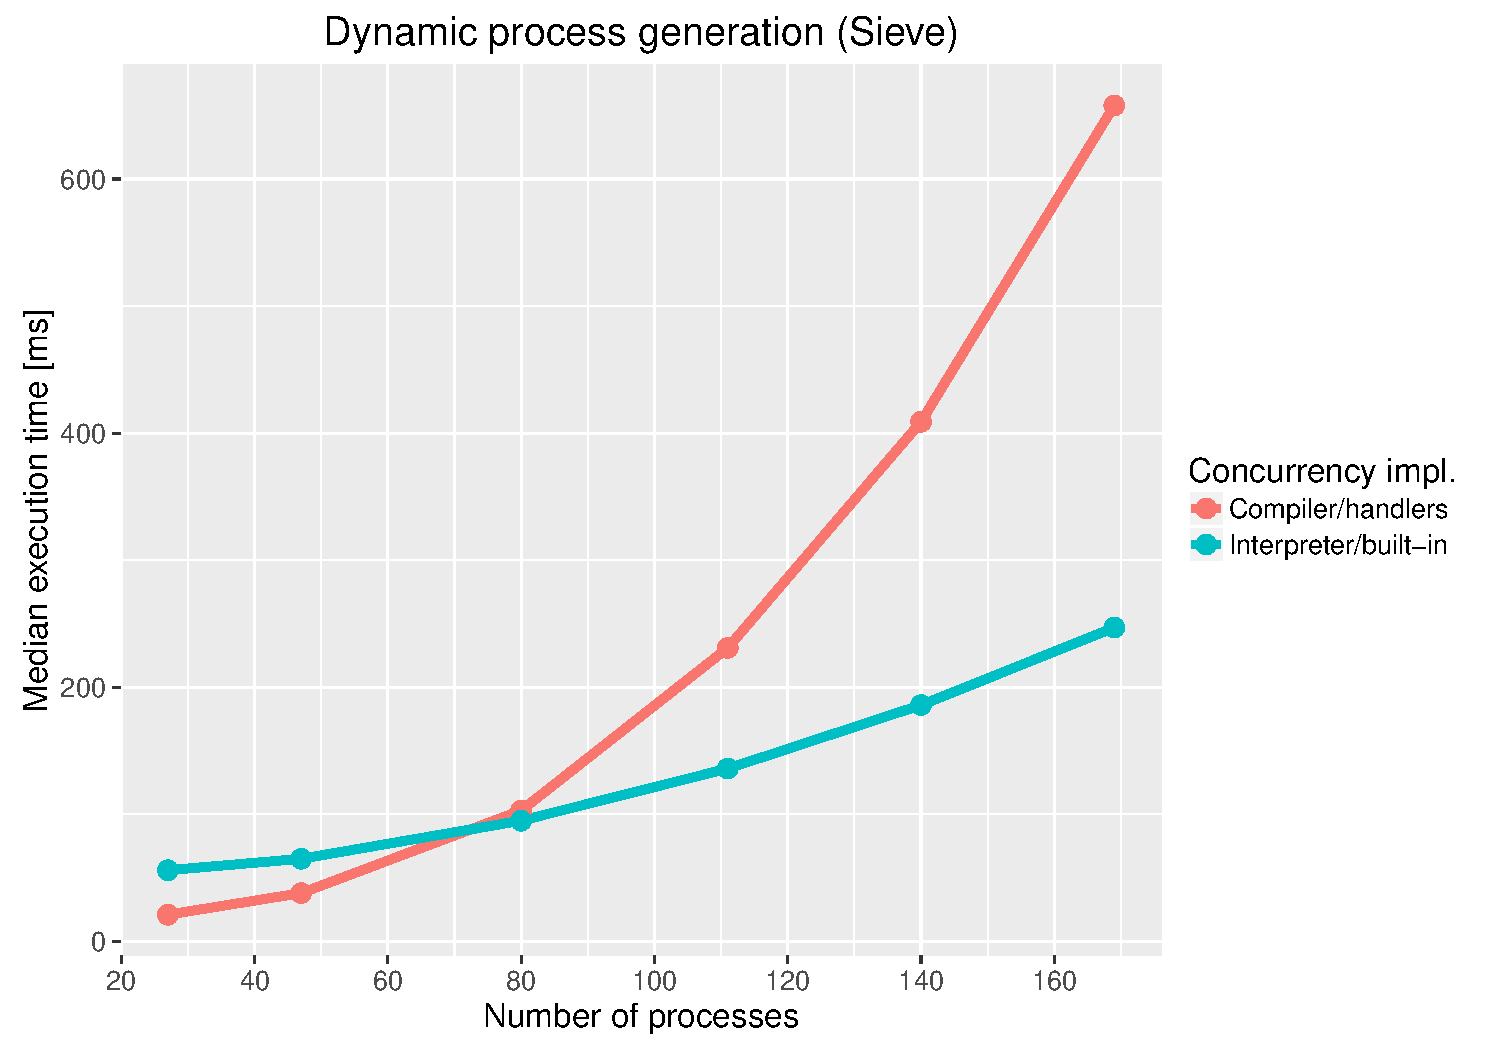
\includegraphics[scale=0.45]{figures/sieve_compiler-interpreter.pdf}
  \end{figure}
\end{onlyenv}
%
\begin{onlyenv}<2->
  \begin{figure}
    \centering
    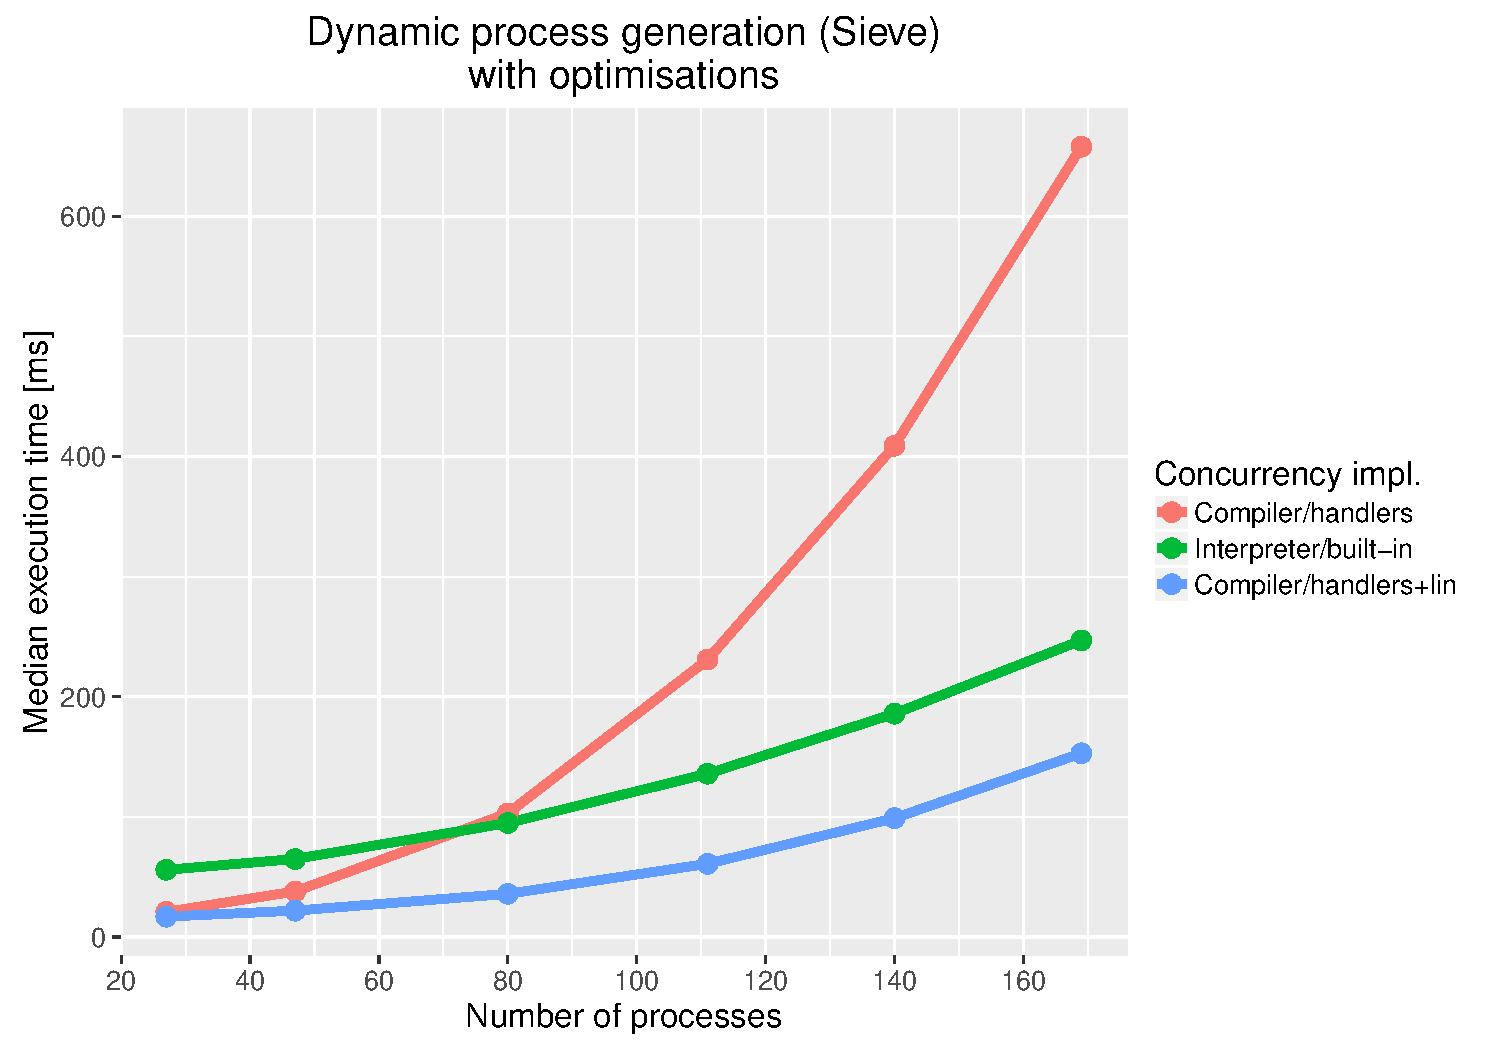
\includegraphics[scale=0.45]{figures/sieve_recovered.pdf}
  \end{figure}
\end{onlyenv}
\end{frame}

%% Tentative schedule
\begin{frame}
  \frametitle{Tentative plan for 2016/17}
\begin{figure}
\centering
\tikzset{every picture/.style={xscale=0.85,transform shape}}
\begin{gantt}{6}{12}
 \begin{ganttitle}
   \titleelement{2016}{4}
   \titleelement{2017}{8}
    \end{ganttitle}
    \begin{ganttitle}
      \titleelement{Sep}{1}
      \titleelement{Oct}{1}
      \titleelement{Nov}{1}
      \titleelement{Dec}{1}
      \titleelement{Jan}{1}
      \titleelement{Feb}{1}
      \titleelement{Mar}{1}
      \titleelement{Apr}{1}
      \titleelement{May}{1}
      \titleelement{Jun}{1}
      \titleelement{Jul}{1}
      \titleelement{Aug}{1}
    \end{ganttitle}
    \ganttbar{P1 (PLDI)}{0}{3}
    \ganttbar{P2 (ICFP)}{2}{5}
    \ganttbar{P3 (TBD)}{6}{6}
    \ganttbar{I (TBD)}{9}{3}
%    \ganttbar{Teaching Assistant for CT}{0}{4}
%    \ganttbarcon{Teaching Assistant for COPT}{4}{2}
  \end{gantt}
\end{figure}
\begin{description}
  \item[P1] Parallel load balancing with handlers and MPI (PLDI).
  \item[P2] Handlers for concurrency in dynamic languages (ICFP).
  \item[P3] Type-and-effect directed optimisations for handlers.
  \item[I] Potential internship.
\end{description}
\end{frame}

% Load subsequent slides, e.g.
%\section{Introduction}
Points:
\begin{itemize}
  \item Multicore OCaml has handlers but not an effect system
  \item Monads and monad transformers are powerful, but not really flexible, e.g. monad transformer gymnastics.
\end{itemize}

% Bibliography
\bibliographystyle{unsrt}
\begin{frame}[allowframebreaks]
  \frametitle{References}
  \bibliography{progression}
\end{frame}
\end{document}
